\dev{Emile Martinez}{}

\textit{Construction de solutions au problème du RDV}

\paragraph{Objectif} Synchroniser n fils d'exécution

\begin{com}
	Eventuellement dire que la def plus formelle est dans le cours, si elle est écrit. Eventuellement aussi la rappeler, pour dire que y a deux phases, et que la phase 2 commencent quand tous les fils ont fini la phase 1
\end{com} 

\begin{minipage}{0.7\linewidth}
	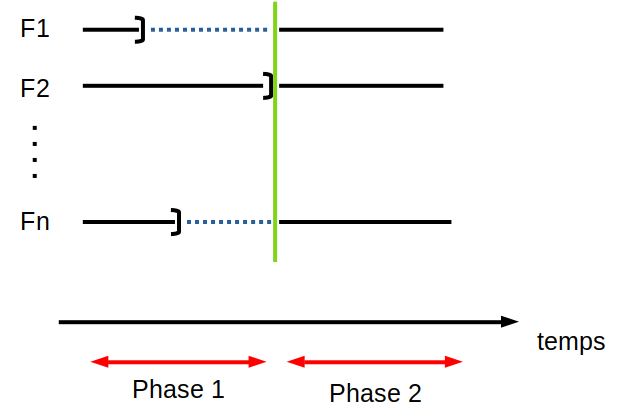
\includegraphics[scale=0.5]{Developpements/probleme du rdv/cas_gen.png}
\end{minipage}
\begin{minipage}{0.3\linewidth}
	\paragraph{But :} Créer la barrière verte
\end{minipage}

\begin{minipage}{0.5\linewidth}
Version naive :
\begin{lstlisting}
int compteur = 0;

    Fi :
	
// Phase 1
compteur ++;
while(compteur <n);

// Phase 2
\end{lstlisting}
\end{minipage}


\begin{minipage}{0.5\linewidth}
	\begin{com}
		Dire à l'oral que chaque fils dit qu'il a finit puis attend que tout le monde ait finit, que compteur c'est simplement le nombre de fils qui ont fini.
	\end{com}
\end{minipage}

\paragraph{Remarque}\begin{enumerate}
	\item On a un problème d'accès conccurent à compteur
	\item On a de l'attente active
\end{enumerate}

\begin{com}
	Mentionner le fait que l'accès conccurent on pourrait simplement mettre un verrou, mais que pour l'attente active c'est plus pénible.
\end{com}

\paragraph{1ere cas facile} Voyons le cas où on a seulement deux fils et où l'on sait que c'est F1 qui finit en premier. On peut alors considérer que F2 n'a pas de phase 1.\\

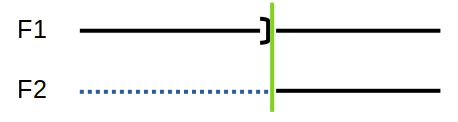
\includegraphics[scale=0.5]{Developpements/probleme du rdv/premier_cas.png}\\

\begin{lstlisting}
sem s <@initialisé à 0@>

    F1:                       F2:
                               
//Phase 1                 decrementer(&s)
incrementer(&s)           //Phase 2
//Phase 2
\end{lstlisting}

\paragraph{2ème cas} T1 finit en dernier mais on a n fils\\

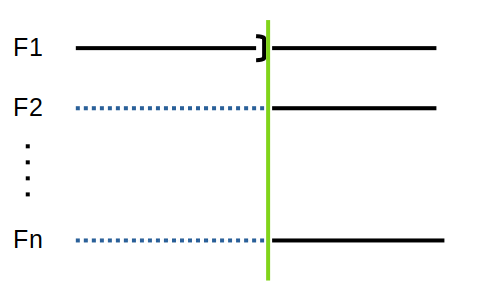
\includegraphics[scale=0.5]{Developpements/probleme du rdv/deuxieme_cas.png}\\

\begin{minipage}{0.6\linewidth}
\begin{lstlisting}
sem s <@initialisé à 0@>

    F1 :                      Fi:
    
// Phase 1                decrementer(&s)
incrementer(&s)           incrementer(&s)
// Phase 2                // Phase 2
\end{lstlisting}

\end{minipage}
\enspace
\begin{minipage}{0.35\linewidth}
\begin{com}
	On reprend la même idée que avant. Mais on veut libérer plusieurs fils. On fait alors en sorte que chaque fil en libère un autre. On obtient ainsi des libérations en cascades
\end{com}
\end{minipage}

\paragraph{Retour au cas général :} On reprend la même idée mais en essayant de bloquer que les fils qui ne sont pas les derniers.
\begin{com}
	On a maintenant besoin de savoir qui termine en dernier. Pour cela, comme chaque fil, attend d'être libéré, on va faire en sorte que seul le dernier fil puisse être libéré. On a qu'a pour cela avoir un sémaphore initialement négatif, qui ne passera positif que pour le dernier fil.
\end{com}

\begin{minipage}{0.5\linewidth}
\begin{lstlisting}
  sem s <@initialisé à -n+1@>

      Fi :

  // Phase 1
1 incrementer(&s)
2 decrementer(&s)
3 incrementer(&s)
  // Phase 2
\end{lstlisting}
\end{minipage} \enspace
\begin{minipage}{0.45\linewidth}
	\begin{com}
		Dire que la première fois que s va devenir strictement positif, c'est quand le n-ième (donc dernier) fil va incrementer s, puis qu'ensuite c'est la même chose que tout à l'heure.
	\end{com}
\end{minipage}

\begin{example}
	Imaginons que l'on ait 3 fils qui exécute ce code
	\begin{center}
		\begin{tabular}{c|c|c|c}
			F1 & F2 & F3 & s\\
			$|$ & $|$ & $|$ & -2\\
			1 & $|$ & $|$ & -1\\
			2 & $|$ & $|$ & -1\\
			$\vdots$ & 1 & $|$ & 0\\
			$\vdots$ & 2 & $|$ & 0\\
			$\vdots$ & $\vdots$ & 1 & 1\\
			$\vdots$ & $\vdots$ & 2 & 0\\
			$\vdots$ & $\vdots$ & 3 & 1\\
			$\vdots$ & 2 & $|$ & 0\\
			$\vdots$ & 3 & $|$ & 1\\
			2 & $|$ & $|$ & 0\\
			3 & $|$ & $|$ & 1\\
			
		\end{tabular}
	\end{center}
\end{example}

\begin{rem}
	On peut ne pas avoir le droit d'utiliser un sémaphore négatif (dont la définition dit qu'il réveille un fil quand on l'augmente et qu'il passe postif)
\end{rem}

\paragraph{Solution} Mélanger la solution précédente et la solution naïve.

\begin{com}
	En effet, dans la naive on arriver à savoir qui était le dernier fils, mais on arriver pas à faire attendre correctement, et là c'est l'inverse.
\end{com}

\begin{lstlisting}
sem s initialisé à 0
compteur = 0
verrou v_c

    Fi :

//Phase 1
prendre(v_c)
compteur ++;
if (compteur == n){
	rendre(v_c)
	incrementer(&s)
}
else{
	rendre(v_c)
	decrementer(&s)
	incrementer(&s)
}
//Phase 2
\end{lstlisting}

\begin{rem}
	Ici, chaque fil en libère un autre, faisant une longue chaine de libération.\\\\
	\begin{tikzpicture}[->, node distance=2cm]
		\node[state] (q0) {Fi1};
		\node[state, right of = q0] (q1) {$Fi2$};
		\node[state, right of = q1] (q2) {$Fi3$};
		\node[state, right of = q2] (q3) {$Fi4$};
		\node[right of = q3] (q4) {};
		\draw (q0) edge[] node{} (q1) ;
		\draw (q1) edge[] node{} (q2) ;
		\draw (q2) edge[] node{} (q3) ;
		\draw (q3) edge[] node{} (q4) ;
		\end{tikzpicture}
		
	\begin{com}
		Si on a beaucoup de coeur et beaucoup de fils, que l'on veut qu'il redémarre tous en même temps vraiment, ca peut poser problème. On a supposé nous que les instructions là était courte par rapport à la phase de travaille, mais ca peut en pas être le cas si jamais on répète beaucoup de fois cette phase de rendez-vous
	\end{com}

	On pourrait préférer alors une libération plus arborescente \\\\
	\begin{tikzpicture}[->, node distance=2cm]
	\node[state] (q0) {Fi1};
	\node[state, above right =1.5cm and 1cm of q0] (q1) {$Fi2$};
	\node[state, below right = 1.5cm and 1cm of q0] (q2) {$Fi3$};
	\node[state, above right of = q1] (q3) {$Fi4$};
	\node[state, below right of = q1] (q4) {$Fi5$};
	\node[state, above right of = q2] (q5) {$Fi6$};
	\node[state, below right of = q2] (q6) {$Fi7$};
	\draw (q0) edge[] node{} (q1) ;
	\draw (q0) edge[] node{} (q2) ;
	\draw (q1) edge[] node{} (q3) ;
	\draw (q1) edge[] node{} (q4) ;
	\draw (q2) edge[] node{} (q5) ;
	\draw (q2) edge[] node{} (q6) ;
	\end{tikzpicture}
\end{rem}

\begin{rem}
	Ici notre sémaphore termine avec comme valeur 1. On pourrait vouloir le réutiliser pour pouvoir faire une nouvelle barrière. On peut alors remplacer la libération en cascade par seulement le premier fil qui libère tout le monde :
	
	\begin{lstlisting}
for(int i = 0; i < n-1; i++) incrementer(&s) 
	\end{lstlisting}
	
	De plus, en gardant le verrou de compteur, on peut empêcher que le rendez vous des phases 2 et 3 interfère avec celui de la phase 1 et 2.
\end{rem}

\begin{rem}
	On pourrait vouloir faire se réunir les fils avec des joins, mais cela impose de tuer les fils (or nous on les conserve) et cela ne s'appliquerait pas à différents processus (ce que permet notre implémentation avec sémaphore).
\end{rem}
